\documentclass{article}
\title{Complexity Matters for Boolean Circuits}
\author{Sam Barrett}

\usepackage{amssymb,amsmath,graphicx}


\begin{document}
    \section{\texttt{EXACT} functions}

    We define the set of functions $\texttt{EXACT}_{k}^{n} : { 0,1 }^{n} \rightarrow { 0,1 } $ as:

    \[
      \texttt{EXACT}_{k}^{n}(x_{1}, \ldots, x_{n}) = 1 \Longleftrightarrow \text{precisely } k \text{ of } x_{1},\ldots,x_{n} \text{ are } 1
    \]

    These functions also satisfy the following recurrence:

    \[
      \texttt{EXACT} _{k}^{1}(x_{1}) = \begin{cases}
        \neg x_{1} & k=0 \\
        x_{1} & k=1\\
        x_{1} \wedge \neg x_{1} & \text{otherwise}
      \end{cases}
    \]

    With an inductive case defined as follows:

    \[
      \texttt{EXACT}_{k}^{n+1}(\vec{x}, x_{n+1}) = (x_{n+1}\wedge \texttt{EXACT}_{k-1}^{n}(\vec{x}) \vee (\neg x_{n+1} \wedge \texttt{EXACT}_{k}^{n}(\vec{x}) ))
    \]

    Here we essentially do a case analysis on a newly introduced variable $x_{n+1}$, the LHS of the disjunction states: if $x_{n+1}$ is 1, then to satisfy $\texttt{EXACT}_{k}^{n+1} $, we must have $k-1$ 1s (true values) in the remaining variables $\vec{x}$. Alternatively on the RHS of the disjunction, we say if $x_{n+1}$ is false, there must be exactly $k$  1s in $\vec{x}$ in order to satisfy $\texttt{EXACT}_{k}^{n+1} $.


    We can show that circuits computing $\texttt{EXACT}_{k}^{n} $ ($\texttt{EX}_{k}^{n} $) are polynomial in $n$ and $k$:

    \begin{figure}[ht]
      \centering
      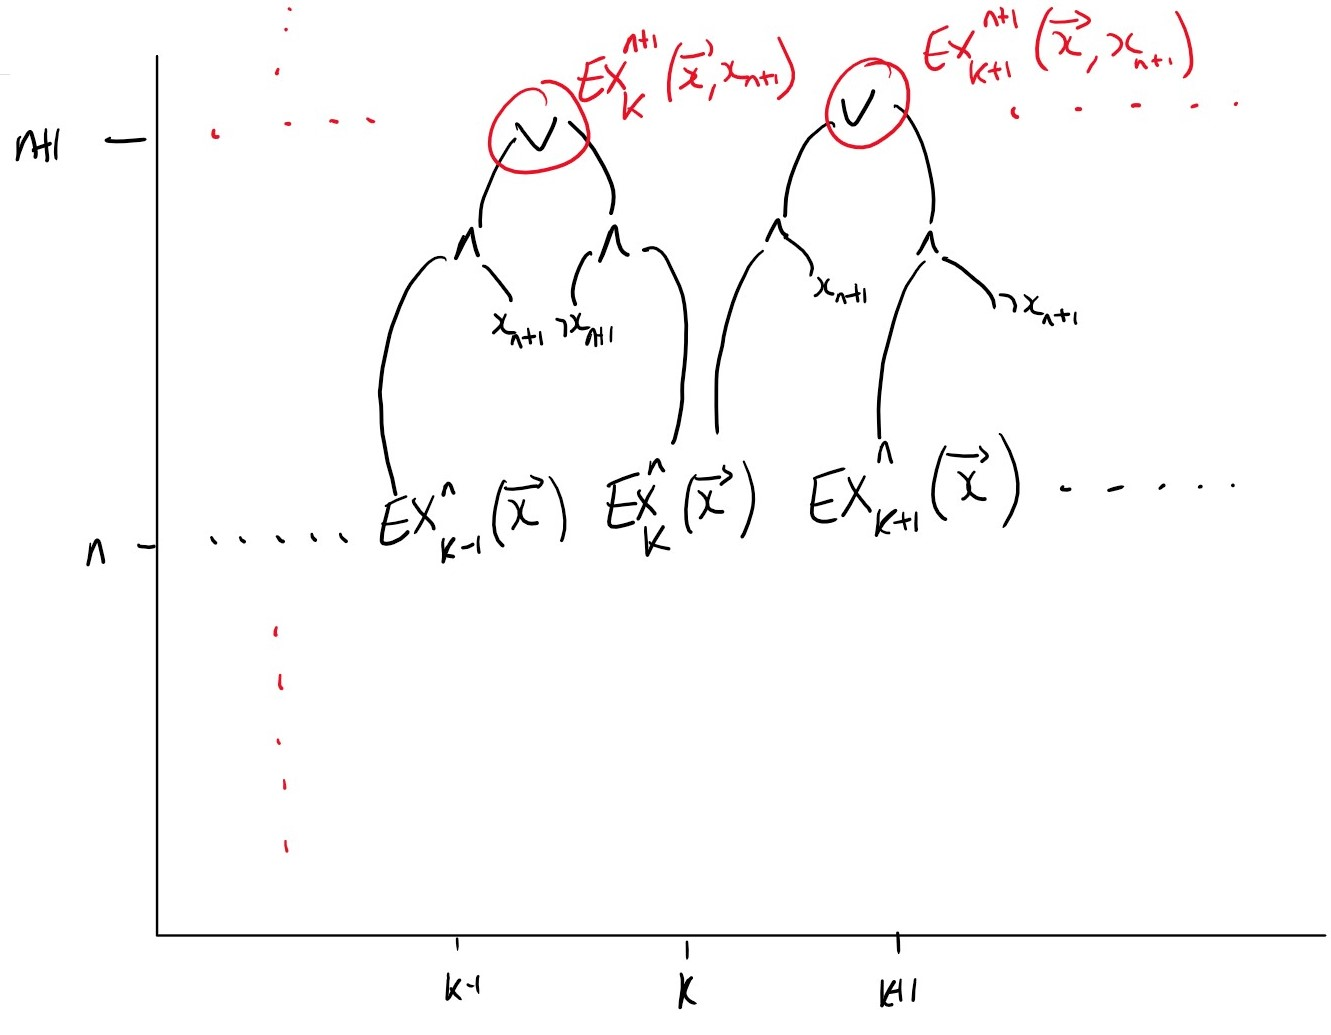
\includegraphics[scale=0.4]{figures/polycircuits}
      \caption{\label{fig:polycircuits} Polynomial-size circuits for $\texttt{EXACT}_{k}^{n} $}
    \end{figure}

    In Figure~\ref{fig:polycircuits} you can see that we can construct our inductive case for any $n$ and $k$. We must be careful to construct all circuits for $k$ before attempting to construct the next layer of $n$.

    Because we only need to consider values of $k$ from $-n$ to $n$ we add a constant number of nodes each time we increase $n$, we can say that this construction is polynomial in size wrt $n$ and $k$.

    \section{Inequality}

    Inequality is known to be non-symmetric. Symmetric boolean functions are boolean functions whose results depend only on the number of 1s in the input.

    We define the $\leq$ relation on natural numbers as $\texttt{LEQ}^{n}: \{ 0,1 \} ^{n} \times \{ 0,1 \} ^{n} \rightarrow \{ 0,1 \} $ by:

    \[
      \texttt{LEQ}^{n} = 1 \Longleftrightarrow \text{number coded by } \vec{x} \leq \text{ number coded by } \vec{y}
    \]


    \begin{align*}
      \texttt{LEQ}^{1}(x,y) &= \neg x \vee y   \\
      \texttt{LEQ}^{n+1}(\vec{x}x_{n+1},\vec{y}y_{n+1}) &= \begin{cases}
        \texttt{LEQ}^{1}(\vec{x},\vec{y}) \wedge \texttt{NEQ}^{n}(\vec{x},\vec{y}) & x_{n+1} \wedge \neg y_{n+1} \\
        \texttt{LEQ}^{n}(\vec{x},\vec{y}) & \text{otherwise}
      \end{cases}
    \end{align*}

    Where $\texttt{NEQ}^{n}(\vec{x},\vec{y}) = 1, iff \vec{x} \neq \vec{y}$. We also know that $\texttt{NEQ}^{n}$ can be computed by linear-size circuits.

    We can again demonstrate the polynomial size of this circuit family computing the $\leq$ relation:

    \begin{figure}[ht]
      \centering
      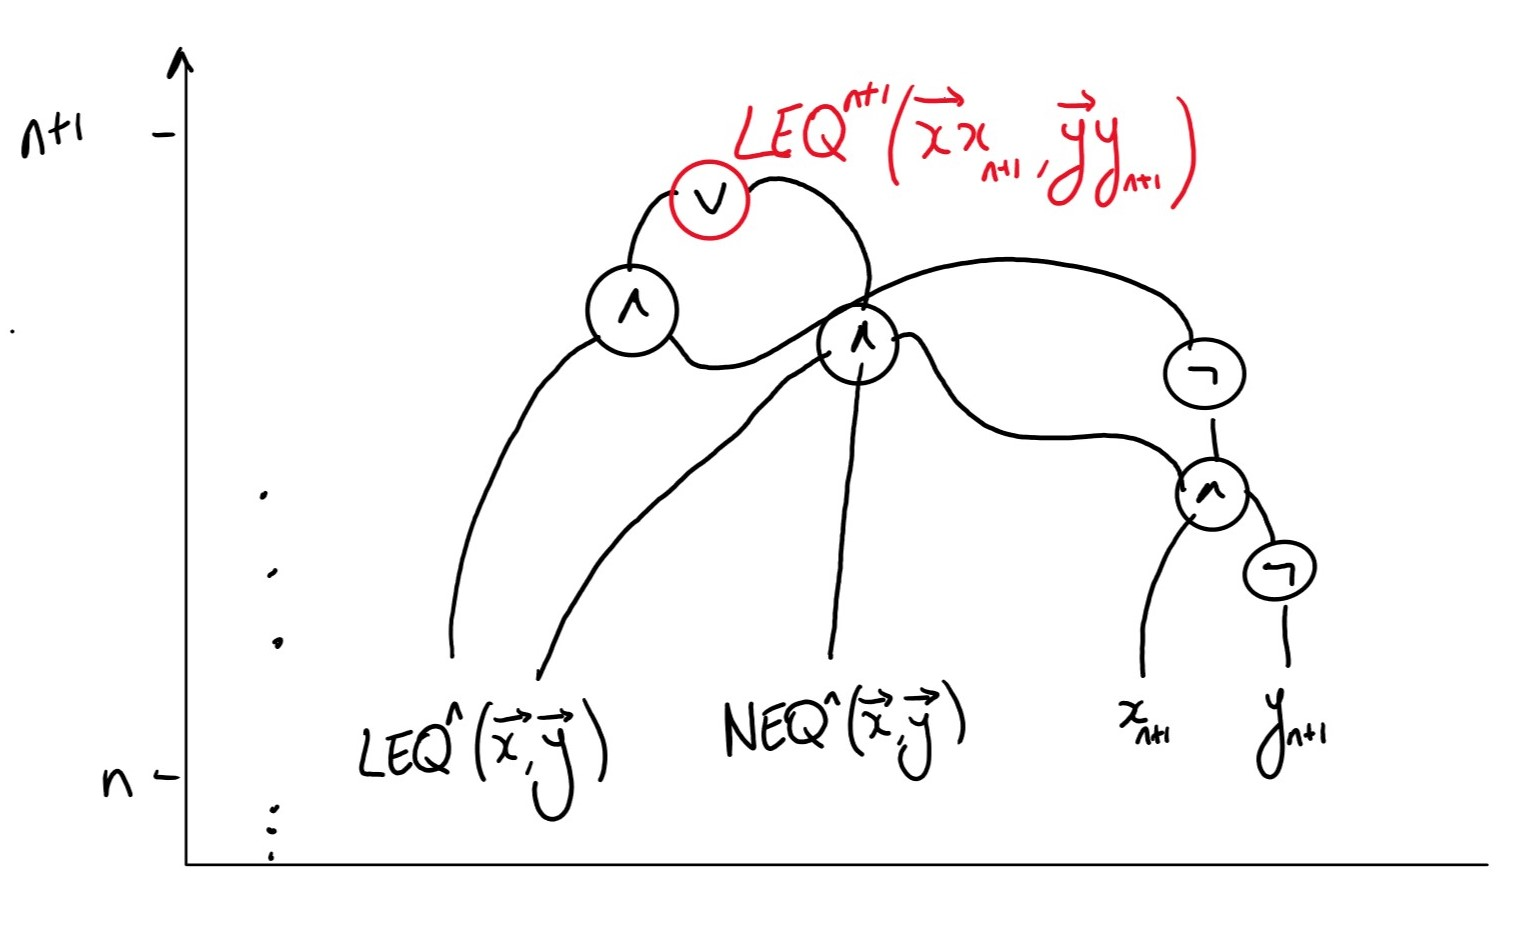
\includegraphics[scale=0.4]{figures/ineqcircuits}
      \caption{\label{fig:ineqcircuits} Polynomial size circuits for inequality}
    \end{figure}


    \section{Composing Constructions}


    We can compose the previous constructions through the use of \textbf{Boolean Connectives} in order to define new circuit families:

    For instance the set $\texttt{ALMOST}_{k}^{n} \subseteq \{ 0,1 \}^{n} $ is the set of binary strings with \textbf{at most} $k$ 1s. It can be computed as follows using our $\texttt{EXACT} $ circuit family:

    \[
      \texttt{EXACT}_{0}^{n}(\vec{x}) \vee \texttt{EXACT}_{1}^{n}(\vec{x})  \vee \ldots \vee \texttt{EXACT}_{k}^{n}(\vec{x})
    \]

    \subsection{Undecidability}

    In the last lecture we saw how we can construct the set $\mathbf{P} \backslash poly$.

    We constructed this set in relation to the length of an input to a function.

    We said that if the length of the input codes a halting Turing machine, it is in $\mathbf{P}\backslash poly $. And more generally defined it as:

\[
  \mathbf{P} \backslash poly := \bigcup_{c=1}^{\infty} \mathbf{SIZE}(n^{c})
\]

We can therefore say that any unary language is in $\mathbf{P}\backslash poly$ as in this case $n=1$. Meaning Any unary language has the possibility of being undecidable.


It can also be shown that $\mathbf{P} \subseteq \mathbf{P}\backslash poly  $. This allows us to recover polynomial sized circuit families for a wide variety of problems.

This also allows us to consider Turing machines as \textit{high level} programs which can be \textit{compiled} to \textit{low level} circuitry with low complexity overhead.
\end{document}
